%!TEX TS-program = pdflatex
\documentclass{emulateapj}

\shorttitle{AQS on MIKE}
\shortauthors{Casey et al}

\begin{document}

\title{The Aquarius Stream Progenitor Was Not a Globular Cluster}


\author{Andrew R. Casey\altaffilmark{1,2}, Stefan C. Keller\altaffilmark{1}, Frebel, Anna\altaffilmark{2}, Gary Da Costa\altaffilmark{1}, Alan Alves-Brito\altaffilmark{1}}
\altaffiltext{1}{Research School of Astronomy \& Astrophysics, Australian National University, Mount Stromlo Observatory, via Cotter Rd, Weston, ACT 2611, Australia}
\altaffiltext{2}{Massachusetts Institute of Technology, Kavli Institute for Astrophysics and Space Research,
77 Massachusetts Avenue, Cambridge, MA 02139, USA}


\begin{abstract}
\end{abstract}

\keywords{Galaxy: halo, structure --- Individual: Aquarius Stream --- Stars: FGK-giants}

\section{Introduction}

Stellar streams in the halo are relics of relatively recent minor mergers in the Milky Way. The positions and kinematics of stars within these streams are sensitive to the galactic potential. As such, they can collectively constrain the chemodynamical evolution of the galaxy, the fraction and distribution of accreted matter in the stellar halo, the sub-halo mass function, as well as the shape and extent of dark matter in the Milky Way. 

Wide field digital image catalogues have proved excellent sources for finding stellar streams. Dozens of streams reaching out up to 150\,kpc in the stellar halo have been identified through photometric selections and matched-filtering techniques. However, as \citet{Helmi;et-al_1999} point out, these methods are only successful for identifying substructures that are sufficiently distant from the solar neighbourhood. A nearby stream within 10\,kpc will not appear as an on-sky over-density. Such an object would only be detectable by utilising both position and kinematic information. 

% Talk about RAVE
It is therefore necessary to survey the kinematics of solar neighbourhood stars in order to detect nearby streams. The RAVE (Radial Velocity Experiment) began such a survey in 2003 and has observed spectra from over 500,000 stars across 17,000 deg$^{2}$. Candidates for RAVE were chosen based only on their apparent magnitude of 9 $<$ I $<$ 13, and therefore are not kinematically biased towards detecting nearby streams. The RAVE data releases have provided radial velocities \citep{Steinmetz;et-al_2006} and estimates of stellar parameters \citep{Zwitter;et-al_2008, Siebert;et-al_2011} now for a subset of these observations. 

% Identification of the aquarius stream
Using this data, \citet{Williams;et-al_2011} identified a co-moving group of nearby ($0.5 \leq d \leq 10$\,kpc) stars in the direction of the Aquarius constellation. The artefact is most apparent when examining kinematics against galactic latitude for stars within $-70\,^\circ < b < -50\,^\circ$. \citet{Williams;et-al_2011} employed a selection criteria of $-250 < V_{hel} < -150$\,km s$^{-1}$, $30\,^\circ < l < 75\,^\circ, J > 10.3$ and identified 15 stream candidates. The average heliocentric radial velocity of these members is $V_{hel} = -199$\,km s$^{-1}$, with a dispersion of 27\,km s$^{-1}$. When compared to other streams identified in the halo, this is an unusually wide kinematic dispersion. Streams are generally considered to be kinematically cold, with dispersions of $\sigma_v < 8$\,km s$^{-1}$. The radial velocities outputted by the RAVE survey are described to be $\sim{}2$\,km s$^{-1}$, so the wide kinematic distribution is not limited by the observational data.

% is it a real substructure
\citet{Williams;et-al_2011} quantified the statistical significance of the Aquarius substructure with comparisons to the Besancon and Galaxia models. After populating the models, the galaxy representations were discretized in $\Delta{}V_{hel}$ and $\Delta{}l$ grid blocks. 

There is no reason to suspect that the Aquarius stream is not a real substructure.

% What is it?
Given the extent of stellar debris the Sagittarius dwarf has littered in the Milky Way, it is reasonable to suspect the Aquarius stream may simply be Sagittarius in origin. Although the metallicities reported by \citet{Williams;et-al_2011} are not dissimilar from the stream, the distances and $V_{Z}$, $V_\phi$ for Aquarius are quite distinct from Sagittarius. \citet{Williams;et-al_2011} concluded that the newly discovered stream could not be positively associated with the Monoceros stream, Hercules-Aquila cloud, or either the Canis Major or Virgo Overdensities.

% MRS follow-up by de boer
In order to investigate the Aquarius progenitor and any possible association with existing substructures, \citet{Wylie-de_boer;et-al_2012} observed six Aquarius stream members with medium resolution (R = 25,000) spectroscopy. Their data indicates the stream is chemically coherant, with a dispersion of only 0.1\,dex. Based on sodium and nickel abundance ratios with respect to iron, they claim the Aquarius stream chemical signatures unambiguously represent those of a globular cluster. Additional abundances of oxygen, magnesium and aluminium are reported to solidify this claim.

% globular cluster chemical signatures

We seek to investigate the globular cluster origin claim made by \citet{wylie-de_Boer;et-al_2012}. We present a detailed chemical abundance analysis for six confirmed Aquarius stream members observed using the Magellan Inamori Kyocera Echelle spectrograph \citep{Bernstein;et-al_2002} on the Magellan telescope. Details of the observations and data reduction are outlined in the following section. The data analysis is presented in \S\ref{sec:analysis} and a detailed discussion of these results resides in \S\ref{sec:discussion}, as well as an alternative hypothesis for the origin of the Aquarius stream. In \S\ref{sec:conclusion} we present our conclusions and critical interpretations.

\section{Observations \& Data Reduction}

The most comprehensive sample of Aquarius stream stars is presented in the discovery paper of \citet{Williams;et-al_2011}. Since the globular cluster origin claim of \citet{de_Boer;et-al_2012} is based from a subset of six of these stars, we targeted stars largely from the sample of \citet{de_Boer;et-al_2012}. An additional star from the original \citet{Williams;et-al_2011} sample, J2306265-085103, was also observed. Program stars were observed in July 2011 and we used standard stars observed for a separate program in March 2011. All standard and program observations were observed using the 1.0" slit, which provides a spectral resolution of $R = 28,000$. The exposure times for our program stars varied per star from X seconds to Y seconds, providing a signal-to-noise in excess of 100 per pixel element at 600 nm for all stars.

The data were reduced using the CarPy pipeline. Standard ThAr arc lamp exposures were taken to provide wavelength calibration. Quartz and milky flat fields at the start of each night were used. No telluric corrections were made as atmospheric absorption does not affect any of the our lines of interest. Each reduced echelle order was interactively normalised using a third order spline. All orders were then stitched together to provide a full spectral coverage from 3800-9400\,\AA{}. 

\begin{deluxetable*}{lcccccccccc}
\tablecolumns{1}
\tabletypesize{\scriptsize}
\tablecaption{Observations\label{tab:observations}}
\tablehead{
	\colhead{Designation} &
	\colhead{$\alpha$} &
	\colhead{$\delta$} &
	\colhead{Observed} &
	\colhead{Airmass} &
	\colhead{Seeing} &
	\colhead{$t_{exp}$} &
	\colhead{S/N\tablenotemark{a}} &
	\colhead{$V_{rad}$} &
	\colhead{$V_{hel}$} &
	\colhead{$V_{err}$} \\
 & (J2000) & (J2000) & Date & & (") & (secs) & (px$^{-1}$) & (km s$^{-1}$) & (km s$^{-1}$) & (km s$^{-1}$)
}
\startdata

C2225316-14437	& 22:25:31.7 & $-$14:54:39.6	& 2011-07-30	& 1.033 & \dots & \dots & \dots & $-$169.0	& \dots & 0.7 \\
C2306265-085103	& 23:06:26.6 & $-$08:51:04.8	& 2011-07-30	& 1.096 & \dots & \dots & \dots & $-$239.3	& \dots & 0.6 \\
HD41667			& 06:05:03.7 & $-$32:59:36.8	& 2011-03-13	& 1.005	& \dots & \dots & \dots & 314.4	& \dots & 0.8 \\
HD142948		& 16:00:01.6 & $-$53:51:04.1	& 2011-03-14	& 1.107	& \dots & \dots & \dots & 6.8		& \dots & 0.4 \\
J221821-183424	& 22:18:21.2	& $-$18:34:28.3	& 2011-07-30	& 1.026	& \dots & \dots & \dots & $-$170.5	& \dots & 0.5 \\
J223504-152834	& 22:35:04.5	& $-$15:28:34.9	& 2011-07-30	& 1.047	& \dots & \dots & \dots & $-$180.9	& \dots & 0.7 \\
J223811-104126	& 22:38:11.6	& $-$10:41:29.4	& 2011-07-30	& 1.218	& \dots & \dots & \dots & $-$248.4	& \dots & 0.7 

\enddata
\tablenotetext{a}{S/N measured at 6000 \AA{} for each target.}
\end{deluxetable*}


\section{Analysis}
\label{sec:analysis}

\subsection{Radial Velocities}
\label{sec:radial-velocities}
The radial velocity for each star was determined in a two-step method. An initial estimate of the radial velocity was ascertained by cross-correlation with a synthetic spectrum of a giant with $T_{eff} = 4500$\,K, $\log{g} = 1.5$, and [M/H] $= -1.0$ across the wavelength range $8450 - 8700$ \AA{}, allowing us to place our spectrum at pseudo-rest. Velocities found from cross-correlation are typically within 1\,km\,s$^{-1}$ of our final published value.

The equivalent widths for $\sim{}N$ absorption lines were measured, allowing for the radial velocity of each line to be calculated from the ratio of laboratory and rest wavelengths. The final radial velocity is then given by the mean of these $\sim{}N$ measurements. Figure \ref{fig:line-velocities} shows the line velocities for HD440077 after  being placed at rest using our cross-correlation velocity of X.XX\,km s$^{-1}$. As expected, the mean offset is small ($-1.1$\,km s$^{-1}$), and our standard deviation is X.XX\,km s$^{-1}$ from N line measurements. This provides us with a final measured radial velocity of $X.XX \pm X.XX$\,km s$^{-1}$. This process was repeated for all standards and observations. The radial velocities published in Table \ref{tab:observations} are the final values from this two-step method. Heliocentric velocities agree excellently () with previously reported literature values \citep{Williams;wylie-de_boer;2012}.

\subsection{Line Measurements}
\label{sec:line-measurements}

For the measurement of atomic absorption lines, we employed the line list of \citet{Yong;et-al_2009} with additional transitions of Cr, Sc, Zn, and Sr from \citet{Frebel;et-al_2009}. Molecular line data for CH was taken from \citet{Plez;et-al_2008,Plez;et-al_2009}. We further supplemented the list with hyperfine-structure data for Sc and Mn  from the Kurucz compilation \citet{Kurucz;1998}. For lines with hyperfine structure, blended transitions or molecular features, we used a spectral synthesis approach. The abundance of a given species was obtained by matching a synthetic spectrum of known abundance to the observed spectrum.

We list the atomic data and measured equivalent widths for atomic lines used during this analysis in Table \ref{tab:equivalent-widths}. In order to exclude saturated lines we only used lines with a reduced equivalent widths $\log_{10}{(\mbox{EW}/\lambda)} < -4.5$ in our chemical abundance analysis. A minimum detectable equivalent width was measured as a function of wavelength, and only lines that exceeded a $3\sigma$ detection significance were included. We have verified our equivalent width measurement techniques by measuring equivalent widths for N lines in HD140283 and comparing our measurements with the study of \citet{Norris;et-al_2000}. Excellent agreement is found between the two studies, which is illustrated in Figure \ref{fig:ew-compare}. The mean difference between this study and that of \cite{Norris;et-al_2000} is a negligible $0.64 \pm 2.78$\,m\AA{}, and no systematic trend is present.

% equivalent widths plot with Norris for HD 122563
\begin{figure}[h]
	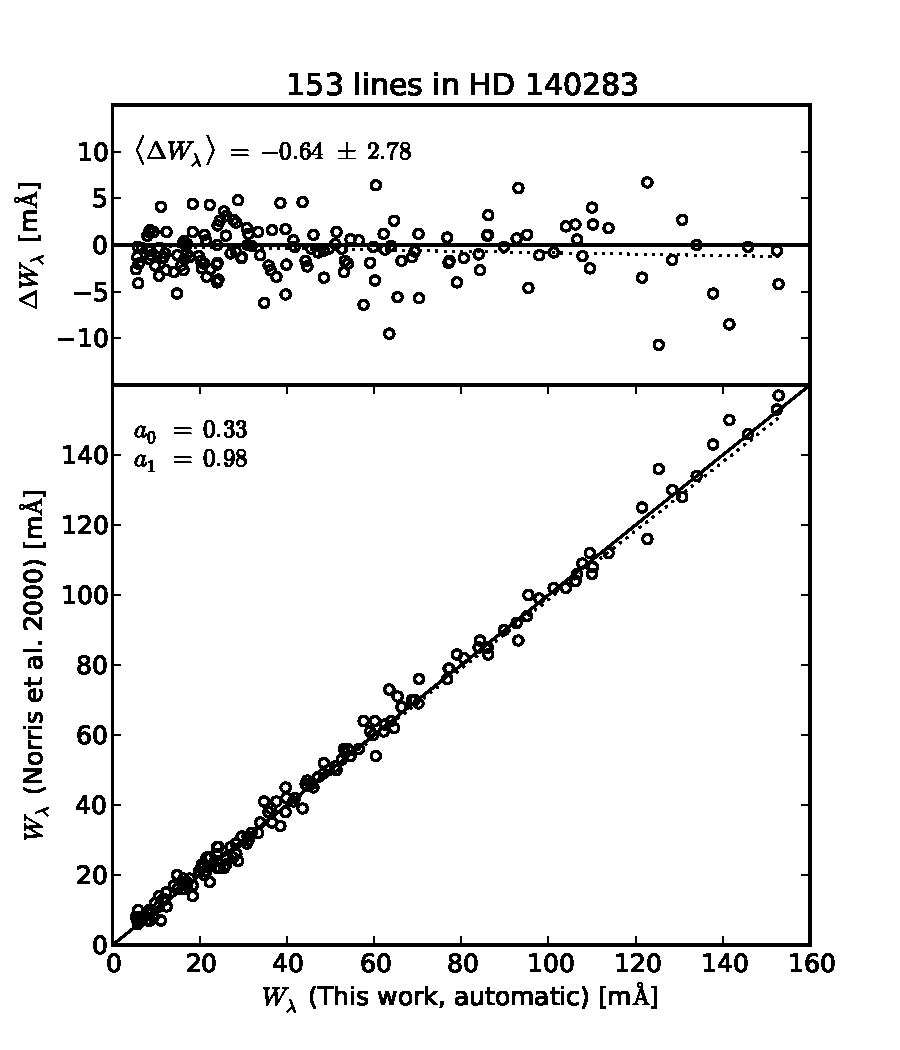
\includegraphics[width=\columnwidth]{./figures/smh-norris.pdf}
	\caption{The gold standard comparison.}
	\label{fig:ew-compare}
\end{figure}

% equivalent widths table

\subsection{Model Atmospheres}
We employed the ATLAS9 stellar atmospheres of \citet{Castelli;Kurucz_2003} for this analysis. These one-dimensional models ignore any centre-to-limb spatial variations, assume local thermodynamic equilibrium as well as overall hydrostatic equilibrium, and assumes no convective overshoot from the photosphere. The stellar parameter spacing for these grid models is 250\,K, 0.5 dex in surface gravity, 0.5 dex in [M/H] and 0.1 dex in [$\alpha$/Fe]. We interpolated the stellar densities, temperatures, electron pressures at all stellar depths between atmospheres using the Quickhull algorithm during our analyses. Quickhull is reliant on Delaunay tessellation, which suffers from extremely skewed cells when the grid points vary in size by orders of magnitude -- as $T_{eff}$ values do compared to $\log{g}$ or [M/H]. If unaccounted for, these asymmetric cells can manifest as non-negligible errors in interpolated densities, temperatures, pressures, and opacities across all photospheric depths. We scaled each stellar parameter between zero and unity prior to interpolation to minimise these errors. During this step, $\log{g}$, [Fe/H] and [$\alpha$/Fe] points were scaled such that we simultaneously interpolate linearly in $T_{eff}$ and logarithmically in all other parameters.

\subsection{Stellar Parameters}
The most recent version of the spectral synthesis code MOOG \citep{Sneden;et-al_1973} has been used to derive individual line abundances and stellar parameters. This version employs a more accurate treatment of Rayleigh scattering \citet{Sobeck;et-al_2011}, which is particularly important for transitions blueward of 450\,nm. This is noteworthy, but is less relevant for this analysis as most of our line measurements blueward of 450\,nm are too blended and not used. We have scaled our abundances to solar values using the abundances of \citet{Asplund;et-al_2009}.

The effective temperature for each star was found by demanding a zero-trend in excitation potential and abundance for each measured Fe\,I line. In the same way, the microturbulence was found by demanding a zero trend in reduced equivalent width against abundance. Linear relationships with slopes of $|0.005|$ dex were considered to be converged. Surface gravity was found by forcing the mean Fe\,I and Fe\,II abundances to be equal, whilst maintaining zero trends with the excitation potential, reduced equivalent width and abundance. After these parameters had converged, the model metallicity was exactly matched to that of our line abundances. Line abundances that were unusually deviant ($>3\sigma$) from the mean were removed. The largest number of outlier measurements removed for any observation was N for X.


% spectral plots for five stars

\begin{deluxetable*}{lcccccccccccccc}
\tablecolumns{2}
\tabletypesize{\scriptsize}
\tablecaption{Stellar Parameters}
\tablehead{
	\colhead{Designation} &
	\colhead{$T_{\mbox{eff}}$} &
	\colhead{$\log{g}$} &
	\colhead{$v_t$} &
	\colhead{[Fe/H]} & 
	\colhead{$T_{\mbox{eff}}$} &
	\colhead{$\log{g}$} &
	\colhead{$v_t$} &
	\colhead{[Fe/H]} &
	\colhead{Source} \\
}
\startdata
C2225316-14437	& 4350	& 1.60	& 1.80	& --1.19	
				& 4235 $\pm$ 118 & 1.45 $\pm$ 0.21 & 1.96 $\pm$ 0.11 & --1.20 $\pm$ 0.14 \\
C2306265-085103	& 4180	& 1.00	& 1.80 	& --1.16
				& \dots	& \dots	& \dots	& \dots
				& \dots \\	
HD41667			& 4630	& 1.70	& 1.66 	& --1.21
				& 4605	& 1.88	& 1.44	& --1.16
				& \citet{Gratton;et-al_2000} \\
HD44007			& 4790	& 1.78	& 1.63	& --1.80
				& 4850	& 2.00 	& 2.20	& --1.71
				& \citet{Fulbright_2000} \\
HD142948		& 4950	& 2.19	& 1.78	& --0.79
				& 4713 	& 2.17 	& 1.38	& --0.77
				& \citet{Gratton;et-al_2000} \\
J221821-183424	& 4570	& 0.80	& 1.93	& --1.60
				& 4395 $\pm$ 205 & 1.45 $\pm$ 0.35 & 1.96 $\pm$ 0.18 & --1.15 $\pm$ 0.21
				& \citet{wylie-de-boer;et-al_2012} \\
J223504-152834	& 4620	& 2.15 	& 1.44	& --0.65
				& 4597 $\pm$ 158 & 2.40 $\pm$ 0.14 & 1.47 $\pm$ 0.07 & --0.98 $\pm$ 0.17
				& \citet{wylie-de-boer;et-al_2012} \\
J223811-104126	& 5100	& 3.00	& 1.21	& --1.44
				& 5646 $\pm$ 147 & 4.60 $\pm$ 0.15 & 1.09 $\pm$ 0.11 & --1.20 $\pm$ 0.20
				& \citet{wylie-de-boer;et-al_2012} 
\enddata

\end{deluxetable*}


\subsection{Abundances}

% elemental abundances

% comparison to literature for a given star

% chemical synthesis


\subsection{Distances}
% isochrone fitting

% discuss Williams et al distances


\subsection{Dynamics}

% U, V, W calculations



\section{Discussion}

% RAVE pipeline discrepancies

% wylie de boer discrepancies


\subsection{Stellar Parameter Discrepancies with \citet{wylie-de-boer;et-al_2012}}

We repeated our equivalent-width analysis using the atomic line list supplied in \citet{wylie-de-boer;et-al_2012}. Given the lower spectral resolution and modest signal-to-noise in their study, there are fewer unblended absorption lines available. In fact, there are very few transitions present in their published line list: only 14 Fe\,I lines and 3 Fe\,II lines are available.  The oscillator strengths for these lines were calculated from a reverse spectral analysis using the \citet{Hinkle;et-al_2003} solar atlas. 

% Chemistries for various GC trends

% chemistries - [Ni/Na]

% chemistries - [Al/Mg]

% which GC's do not show these trends

% closest looking globular clusters from Harris catalogue

% could they be displaced thick disk stars?


\begin{deluxetable*}{lccccccc}
\tablecolumns{2}
\tabletypesize{\scriptsize}
\tablecaption{Observed Targets\label{tab:observed-targets}}
\tablehead{
	\colhead{ID} &
	\colhead{$\alpha$} &
	\colhead{$\delta$} &
	\colhead{Air mass} &
	\colhead{S/N\tablenotemark{a}} &
	\colhead{$V_{\mbox{helio}}$} \\
 & (J2000) & (J2000) & & (px$^{-1}$) & (km s$^{-1}$)
}
\startdata


HD130694  			& 14:50:17.1 & --27:57:41.6 & 1.289 & \nodata & \nodata \\
HD170642  			& 18:32:21.0 & --39:42:12.8 & 1.464 & \nodata & \nodata \\
HD180928  			& 19:18:59.6 & --15:32:11.5 & 1.934 & \nodata & \nodata \\
HD181342  			& 19:21:03.9 & --23:37:09.7 & 1.203 & \nodata & \nodata \\
HD187111 			& 19:48:39.3 & --12:07:17.8 & 1.281 & \nodata & \nodata \\
HD210049  			& 22:08:22.8 & --32:59:14.6 & 1.006 & \nodata & \nodata \\
C2225316-145437  	& 22:25:31.7 & --14:54:39.6 & 1.033 & \nodata & \nodata \\
J221821-183424 		& 22:18:21.2 & --18:34:28.3 & 1.026 & \nodata & \nodata \\
J223504-152834 		& 22:35:04.5 & --15:28:34.9 & 1.047 & \nodata & \nodata \\
J223811-104126 		& 22:38:11.6 & --10:41:29.4 & 1.218 & \nodata & \nodata \\
C2306265-085103		& 23:06:26.6 & --08:51:04.8 & 1.096 & \nodata & \nodata \\
HD219615  			& 23:17:10.7 &$+$03:16:51.9 & 1.412 & \nodata & \nodata 
\enddata
\tablenotetext{a}{S/N measured at 6000 \AA{} for each target.}
\end{deluxetable*}





\end{document}
